% last updated in April 2002 by Antje Endemann
% Based on CVPR 07 and LNCS, with modifications by DAF, AZ and elle, 2008 and AA, 2010, and CC, 2011; TT, 2014; AAS, 2016

\documentclass[runningheads]{llncs}

\usepackage{amsmath,amssymb,mathrsfs}
\usepackage{ruler}
\usepackage{color}
\usepackage[width=122mm,left=12mm,paperwidth=146mm,height=193mm,top=12mm,paperheight=217mm]{geometry}

\usepackage{multirow}
\usepackage{graphicx}
\usepackage{subfig}
\usepackage{floatrow}
\usepackage[export]{adjustbox}

\usepackage{pifont}
\newcommand{\cmark}{{\color{green} \ding{51}}}%
\newcommand{\xmark}{{\color{red} \ding{55}}}%


\DeclareCaptionFont{tiny}{\tiny}
\DeclareCaptionFont{scriptsize}{\scriptsize}
\captionsetup[subtable]{labelfont={tiny, bf},textfont=normalfont,singlelinecheck=on}
\captionsetup[subfigure]{labelfont={tiny, bf},textfont=tiny,singlelinecheck=on}

\makeatletter
\def\thesubfigure{\textit{\alph{subfigure}}}
\providecommand\thefigsubsep{.}
\def\p@subfigure{\@nameuse{thefigure}\thefigsubsep}
\makeatother

\usepackage{array}
\newcolumntype{x}[1]{>{\centering\let\newline\\\arraybackslash\hspace{0pt}}m{#1}}
\usepackage{tabulary}
\usepackage{booktabs}

\usepackage{standalone}

\usepackage{siunitx}


\usepackage[acronym]{glossaries}
\newacronym{acr::lod}{LoD}{Level of Detail}
\newacronym{acr::lidar}{LiDAR}{Light Detection And Ranging}
\newacronym{acr::dsm}{DSM}{Digital Surface Model}
\newacronym{acr::elod}{eLoD}{evaluation Level of Detail}

\newcounter{SubFigCounter}
\setcounter{SubFigCounter}{1}

\begin{document}

\pagestyle{headings}
\mainmatter{}
\def\ECCV18SubNumber{***}  % Insert your submission number here

\title{Semantic Evaluation of 3D city models}

\titlerunning{ECCV-18 submission ID \ECCV18SubNumber}

\authorrunning{ECCV-18 submission ID \ECCV18SubNumber}

\author{Anonymous ECCV submission}
\institute{Paper ID \ECCV18SubNumber}

\maketitle

\begin{abstract}
    While automatic production of urban models from airborne data is now standard in industry, practitioners have to check the correctness of 3D models by visual inspection and detect the frequent reconstruction errors at city scale. These operations, which are done by experts, are time-consuming, typically taking two hours per square kilometer and per expert. In this work, we propose an approach for automatically assessing 3D models of buildings. Errors and defects present in 3D models are compiled in a hierarchical, flexible and parameterizable taxonomy. The quality of 3D models is predicted based on their intrinsic geometric properties and, when available, on image and depth data. A feature baseline is presented and tested over dataset containing more that one thousand models. It can detect on average $96\%$ of well represented errors. These results motivates further work devising better feature extraction methods over a more well balanced and rich dataset.
    \keywords{3D urban modeling, Quality assessment.}
\end{abstract}

\section{Introduction}

    3D urban models have a wide application range. They can be used for ludic purposes (video games or tourism) as much as they can be vital in more serious domains (for instance: run-off water and microclimate simulation or urban or security operations planification)~\cite{Biljecki2015},~\cite{Musialski2012}. Therefore, automatic urban reconstruction is the focus of both scientific research and industrial activities. However, the problem is still unsolved~\cite{Musialski2012},~\cite{rottensteiner2014results}. In fact, besides the seamless nature of reconstituted models, current algorithms are greedy in time, lack genericity --- regarding different possible urban scenes --- and produce a great deal of erroneous buildings. As such, human intervention is needed either in interaction within the reconstruction pipeline or as a post-processing clean-up step. The later being a long and tedious task~\cite{Musialski2012}, automatizing urban reconstruction evaluation can be helpful, especially in a production environment.

    This work focuses on evaluating polyhedral building models resulting from urban reconstruction methods. Polyhedral models are more compact than triangle meshes extracted from mutliview images or point clouds. In consequence, these models hold more semantic information as each facet typically corresponds to a fa\c{c}ade, a roof or any well defined morphological building face. In counterpart, they are less efficient considering fidelity to input data. Thus, reconstruction algorithms try to find a compromise between compacity and semantics on one hand, and fidelity on the other. Depending on the spatial resolution of input data, the urban scene in question and the targeted application, the reconstruction result has a certain \gls{acr::lod}~\cite{kolbe2005citygml}. A \acrshort{acr::lod} $1$ model is a simple building extrusion. A \acrshort{acr::lod} $2$ model considers geometric simplification of buildings, ignoring superstructures, such as dormer windows and chimneys. These are taken into account in the next \acrshort{acr::lod} $3$. \acrshort{acr::lod} rational is still subject to much discussion~\cite{2016_ceus_improved_lod}. In consequence, we will stick, from hereon, to the simpler previous \acrshort{acr::lod} description as in~\cite{verdie2015lod}.

     Finding a good reconstruction compromise involves answering some hard problems. However, verifying these solutions could be answered much more easily. This motivates the need for a well suited quality assessment paradigm. Since the models to be diagnosed are well structured, an unrestricted evaluation based on data fidelity metrics, as in~\cite{berger2013benchmark}, is too general. It should also ignore format issues or geometric consistencies as studied in~\cite{ledoux2018val3dity}. In fact, these must have been studied well before this stage. The semantic evaluation will only take into account building semantics through the detection and the categorization of modeling errors that can affect these buildings. The herein defined evaluation can thus be used for:
    \begin{itemize}
        \item \textbf{Building models correction}: automatically or interactively correct building models based on the detected errors;
        \item \textbf{Change detection}: where change can be considered as a modeling error or implicitly detected from other errors.
        \item \textbf{Reconstruction method selection}: based on the comparison of reconstruction algorithms performances on errors of interest over a fixed urban scene;
        \item \textbf{Crowd-sourcing evaluation}: by categorizing user behaviors during crowd sourced modeling and vandalism detection.
    \end{itemize}

    \begin{figure}
        \begin{center}
            \includestandalone[mode=buildnew, width=\textwidth]{graphical_abstract}
            \caption{\label{fig::pipeline} The semantic evaluation paradigm proposal: in addition to the input model topological structure depicted in (b), features are extracted from comparison to heightmaps, as represented by the difference computed between the model altimetry and the \acrshort{acr::dsm} in (c). Images can also used to characterize models by comparing its projected edges to local gradients: \textit{c.f.} (d). Based on the computed features, semantic errors affecting the building are predicted using a pretrained classifier.}
        \end{center}
    \end{figure}

     3D urban reconstruction semantic evaluation has not been thoroughly studied until now. Only one benchmark~\cite{rottensteiner2014results} exists but is not widely used for comparison~\cite{lafarge2012creating},~\cite{nguatem2017modeling},~\cite{li2016boxfitting}. Usually reconstruction evaluation is based on visual inspection~\cite{Durupt2006},~\cite{MacayMoreia2013} or geometric precision indices~\cite{Kaartinen2005} without any localized semantic dimension. This work essentially proposes:
    \begin{itemize}
        \item a new \textbf{error taxonomy}, independent from any reconstruction approach or urban scene;
        \item the formulation of the evaluation problem as a \textbf{supervised classification} one that predicts previously defined errors that can affect the building model;
        \item multimodal \textbf{baseline features} which are extracted from the model to feed a classifier for error prediction;
        \item the \textbf{adaptability and flexibility} of the devised framework compared to different input urban scenes and reconstruction methods.
    \end{itemize}

\section{Related Work}

Quality assessment methods can be classified based on two criteria: their output type or the reference data they use.

\noindent
\textbf{Reference Data Types.}
All quality assessment methods need a reference data to be compared to. Indeed, existing approaches compare the 3D reconstructed building models to:
\begin{itemize}
    \item \textbf{Manually plotted ground truth} data with a higher spatial accuracy. These models can be obtained either through field measurements~\cite{Kaartinen2005},~\cite{vogtle2003quality} with the highest possible precision ($\sigma(\text{error}) \approx \SI{0.05}{\meter}$), or using stereo-plotting~\cite{Kaartinen2005},~\cite{Zeng2014}. However this kind of data is not easily to come by.
    \item \textbf{Raw sensor data}. For instance, models can be compared to \acrfull{acr::lidar} point clouds~\cite{Akca2010},~\cite{lafarge2012creating},~\cite{li2016boxfitting} or aerial images~\cite{boudet2006supervised},~\cite{Michelin2013}. Although these are easier to get than the previous ones, they are low on structural and semantic informations for the sake of evaluation.
\end{itemize}
\noindent
\textbf{Evaluation Output Types.}
The quality assessment methods can produce two kinds of outputs:
\begin{itemize}
    \item \textbf{Geometric fidelity metrics}: they summarize the quality of the whole assessed model. These metrics are computed at different levels: points of interest (such as corners or edge points) average precision~\cite{Kaartinen2005},~\cite{vogtle2003quality}, surface dissimilarity~\cite{Kaartinen2005},~\cite{Henricsson1997},~\cite{Zeng2014},~\cite{lafarge2012creating},~\cite{li2016boxfitting} or volume discrepancy to reference data~\cite{Zeng2014}. These outputs have the drawback of being too general for the special case of urban polyhedral models. Their diagnosis, far from surface reconstruction evaluation~\cite{berger2013benchmark}, needs to pinpoint specific types of errors that can be easily corrected once identified~\cite{OudeElberink2010}.
    \item \textbf{Semantic errors}: they identify topological and geometric errors that affect polyhedral models. One example of such taxonomy is the traffic light paradigm (``correct'', ``acceptable'', ``generalized'' and ``rejected'')~\cite{boudet2006supervised}. However, these errors depend on a vague definition of the ``generalized'' level at which models are rejected. In addition, this taxonomy does not help to localize the model shortcomings. Another solution is to look at the issue at hand through the used reconstruction algorithm perspective. For instance, defects are discriminated in~\cite{Michelin2013} between footprint errors (``erroneous outline'', ``inexistent building'', ``missing inner court'' and ``imprecise footprint''), intrinsic reconstruction errors (``over segmentation'', ``under segmentation'', ``inexact roof'' and ``Z translation'') and ``vegetation occlusion'' errors. In the later methods~\cite{boudet2006supervised},~\cite{Michelin2013}, the evaluation is the result of a supervised classification where predicted classes are defects listed in a taxonomy. Features used for the ensuing classification are extracted from high spatial resolution (\SIrange{20}{25}{\cm}) aerial images and \glspl{acr::dsm} like 3D segments and texture correlation scores comparison. In spite of their semantic contribution for quality evaluation, taxonomies risk overfitting to special urban scenes or some reconstruction algorithm.
\end{itemize}

\noindent
\textbf{Main objective.}
This work aims at devising a suitable quality evaluation paradigm when no reference data or only the less structured ones can be provided. It should also be capable of detecting semantic localized errors independently from the used reconstruction methods or the assessed urban scenes.

\section{Problem Formulation}

To evaluate reconstructed input models, an error taxonomy is established. Depending on the evaluation objectives, we deduce error labels that will be used to predict model defects. Buildings are thus annotated in order to train a supervised classifier model that will be used for prediction on other reconstructed models.

The error taxonomy is \textbf{agnostic} towards reconstructed inputs\footnote{produced using any modeling method over all possible urban scenes} and \textbf{parameterizable}. This flexibility and independence means that, at runtime, the evaluation process does not involve heavy computing. Furthermore, it does not require any heavy reference data aside the annotated objects on which the classifier is trained.

The quality assessment pipeline is also \textbf{modular}. Building models are represented by intrinsic geometric features extracted from the model facets graph. If available, the classifier can also be fed additional depth related features, based on the comparison of the model altimetry and the \acrshort{acr::dsm}, in case of aerial reconstruction, or, in general, any depth map comparison. Last but not least, image information can be incorporated to the pipeline through aerial or street view images.

\subsection{Error Taxonomy}
In order to build a generic and flexible taxonomy, we rely on two criteria for error compilation: the building model \acrshort{acr::lod} and the error semantic level, named henceforth \textit{finesse} (\textit{c.f.} Figure~\ref{fig::taxonomy}). A natural integer is attributed to each \textit{finesse} level. Errors with maximal \textit{finesse} are called \textit{atomic} errors. Multiple \textit{atomic} errors can affect a building model. For instance, topological defects induce, almost always, geometrical ones. In practice, only independently coexisting \textit{atomic} defects are reported. The idea is to provide the most pertinent information to be able to correct a model. \textit{Atomic} errors can thus be correlated heuristically to independent actions that an operator or an algorithm needs to choose to correct building models.

\noindent
\textbf{A general layout.}
The main idea of error hierarchization is to enable modularity in the taxonomy, and thus achieve a strong flexibility towards input urban scenes and desired error precision. A general layout is drawn herein before filling in the detailed error descriptions.

At a first level, model qualifiability is studied. In fact, aside from formatting issues or geometric inconsistencies~\cite{ledoux2018val3dity}, other reasons make building models unqualifiable. For instance, buildings can be occluded by vegetation. In general, input models can be impaired by some pathological cases that are outside our evaluation framework. In consequence, \textit{Qualifiable} models will be distinguished from \textit{Unqualifiable} buildings. This first qualification degree corresponds to the \textit{finesse} equal to $0$.

At the \textit{finesse} level one, a qualifiable building reconstruction correctness is predicted. It is the lowest semantization level at which the evaluation of a model is expressed. It is either \textit{Valid} or \textit{Erroneous}.

Model errors are to be grouped into three families depending on the underlying \acrshort{acr::lod}. The first family of errors (``\textit{Building Errors}'') affects the building in its entirety. It corresponds to an accuracy evaluation at $\acrshort{acr::lod}0\text{ } \cup \text{ }\acrshort{acr::lod}1$. At the next $\acrshort{acr::lod}2$, the family ``\textit{Facet Errors}'' assembles defects that can damage fa\c{c}ade or roof fidelity. The last error family, \textit{i.e.} ``\textit{Superstructure Errors}'', describes errors that involve superstructures modeled at $\acrshort{acr::lod}3$. Only the first two families are represented in figure~\ref{fig::taxonomy}.

Each family contains \textit{atomic} errors of maximal \textit{finesse} equal to $3$. These errors are semantically independent, although they can co-occur in the same building model, in the same error family as much as across different ones. They represent particular topological or geometric defects. Topological errors translate inaccurate structure modeling, while geometric ones raise metric positioning inaccuracies.

A scoring system can be attributed to this taxonomy. Each \textit{atomic} error will be attributed a score based on the quality assessment objective. This integer score, ranging from \SIrange{0}{10}{}, describes the confidence level in the defect presence. At $10$ the error must be certainly detected, compared to $0$ where the error must surely not exist. Errors of lower \textit{finesse} inherit their score from their children. The presence of only one child error implicates the presence of its parent, at least, at the same level of confidence. Hence, the parent error category is attributed the maximum score of its children scores.

At evaluation time, three parameters play a role in determining which error labels to consider:
\begin{itemize}
    \item The first is the \textbf{\acrfull{acr::elod}}. Every reconstruction method targets a certain set of \glspl{acr::lod}. They can then be evaluated at multiple levels. In consequence, when assessing a reconstruction, a \acrshort{acr::lod} must be specified. At a predefined \acrshort{acr::elod}, all error families involving higher order details will be ignored.
    \item Depending on the final use of qualification, a \textbf{finesse} level might be preferred. This second evaluation parameter specifies the appropriate semantic level at which errors will be reported.
    \item The last one is error \textbf{exclusivity}. It is based on family error hierarchization. If errors of a certain \acrshort{acr::lod} family are detected, the ones with higher \acrshort{acr::lod} orders are considered meaningless and thus are not reported.
\end{itemize}

\noindent
\textbf{The aerial reconstruction case.}
  \begin{figure}
        \begin{center}
            \includestandalone[mode=buildnew, width=\textwidth]{taxonomy_tree}
            \caption{\label{fig::taxonomy} The proposed taxonomy illustration. In our case of aerial modeling, only two family errors are depicted. At the \textit{finesse} level $2$, hierarchization is possible: the \textbf{exclusivity} parameter can thus act. It is not the case at the \textit{atomic} errors level that are independent by design. }
        \end{center}
    \end{figure}
This study is, henceforth, narrowed to the aerial reconstruction case. The objective is to reconstruct large urban scenes using aerial images or, if available, \acrshort{acr::lidar} point clouds. We will use these data  to confront with the modeled buildings.

In the present case, $2.5$D buildings are evaluated. The next \textit{atomic} errors are proposed:
	\begin{itemize}
		\item \textbf{Building errors} family (\textit{c.f.} Figure~\ref{fig::bul_err}):
        \begin{itemize}
        	\item Under segmentation: two or more buildings are modeled as one;
            \item Over segmentation: one building is subdivided into two or more buildings;
            \item Inexact footprint: erroneous building footprint, grouping geometric inaccuracies and topological defects as missing inner courts ($\equiv$ not the right number of polygon holes);
            \item Imprecise height: wrong building height estimation;
        \end{itemize}
		\item \textbf{Facet errors} family (\textit{c.f.} Figure~\ref{fig::fac_err}):
        \begin{itemize}
        	\item Under segmentation: two or more facets are modeled as one;
            \item Over segmentation: one facet is subdivided into two or more facets;
            \item Inexact segmentation: facet edges are inaccurate;
            \item Imprecise slope: wrong facet slope estimation.
        \end{itemize}
	\end{itemize}

Figure~\ref{fig::samples} illustrates these errors. In (\ref{fig::bul_err}.(a)), Two distinct buildings can be identified visually while they are grouped into one building. The contrary happens when a single building is subdivided in three parts as in (\ref{fig::bul_err}.(b)). The Inexact footprint can be detected easily when it ensues a wrong outline as illustrated in the top right corner of (\ref{fig::bul_err}.(c)). Depth information is hard to convey using images, as shown in (\ref{fig::bul_err}.(d)), where the balcony, besides being detached form its building, has its height wrongly estimated due to the influence of the main building. It is also impossible to deduce the slope mis-evaluation without a depth map as depicted in (\ref{fig::fac_err}.(d)). Another fidelity error can be seen in (\ref{fig::fac_err}.(c)), as the central edge that links the two main roof sides does not correspond to the image position. Facets can also suffer from over segmentation as both roof sides are in (\ref{fig::fac_err}.(b)). To complete the picture, (\ref{fig::fac_err}.(a)) offers a depiction of how a model roof facet can be under segmented.

    \thisfloatsetup{heightadjust=object}
    \begin{figure}
        \begin{center}
            \ffigbox{
                \ffigbox[\FBwidth]
                {
                    \begin{subfloatrow}[4]
                        \ffigbox[\FBwidth]{\caption{Under segmentation}\label{fig::under_bul}}{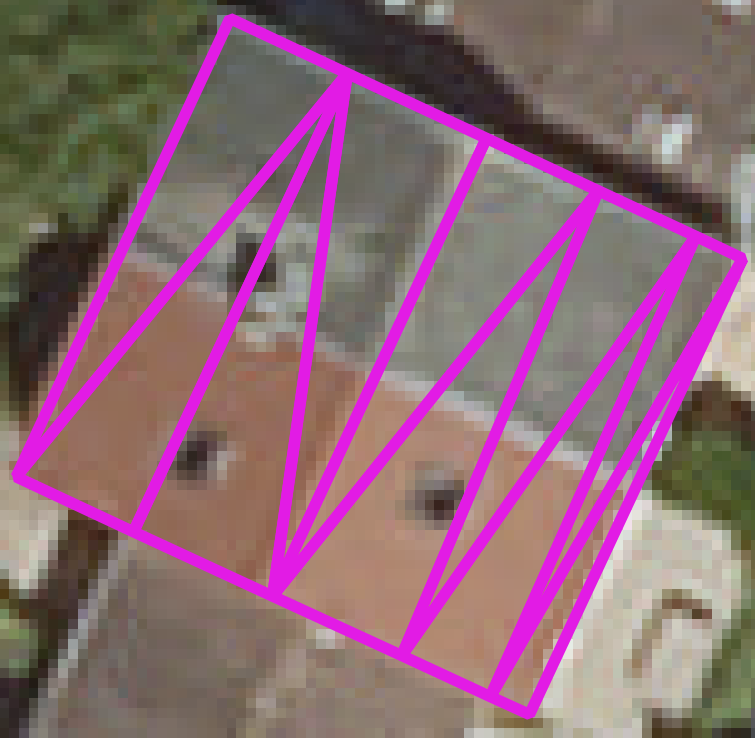
\includegraphics[height=.11\textheight]{images/Building_Errors/under_segmentation}}
                        \ffigbox[\FBwidth]{\caption{Over segmentation}\label{fig::over_bul}}{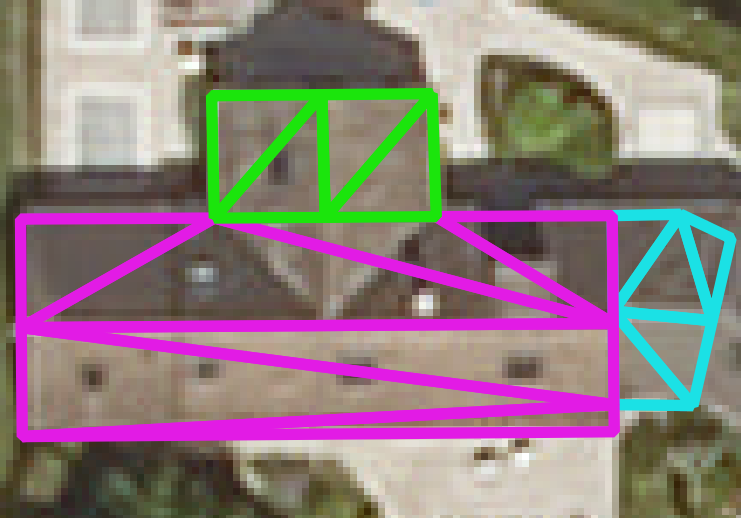
\includegraphics[height=.11\textheight]{images/Building_Errors/over_segmentation}}
                        \ffigbox[\FBwidth]{\caption{Inexact footprint}\label{fig::footprint}}{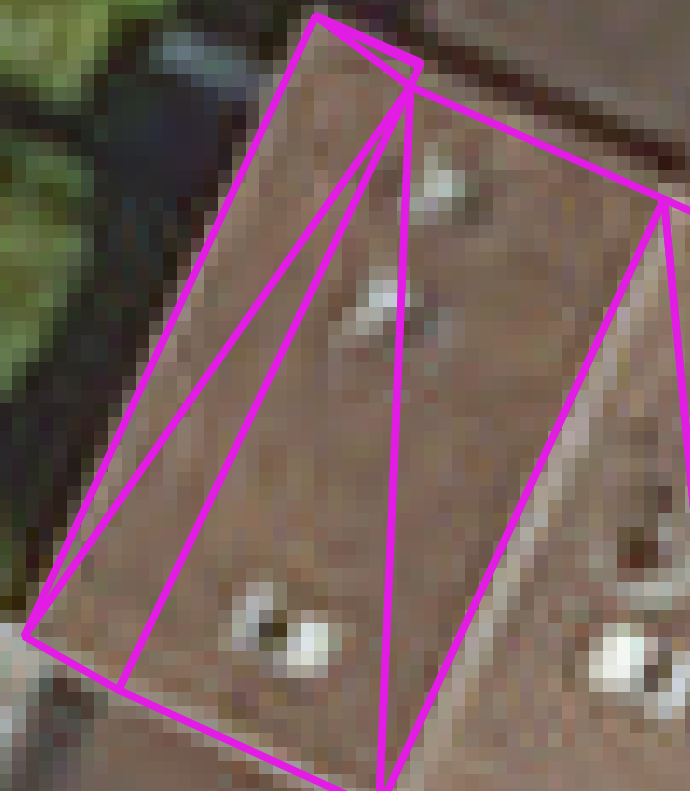
\includegraphics[height=.11\textheight]{images/Building_Errors/footprint}}
                        \ffigbox[\FBwidth]{\caption{Imprecise height}\label{fig::too_low}}{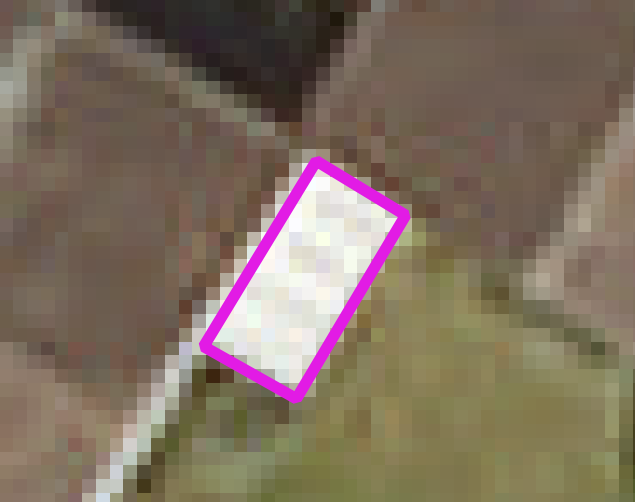
\includegraphics[height=.11\textheight]{images/Building_Errors/altimetric}}
                    \end{subfloatrow}
                }
                {
                    \captionsetup{labelfont={tiny, bf},textfont=scriptsize,justification=raggedright, labelsep=period}
                    \renewcommand{\thesubfigure}{\roman{SubFigCounter}}

                    \captionof{subfigure}{Building errors family samples.}\label{fig::bul_err}
                    \refstepcounter{SubFigCounter}
                    \addtocounter{figure}{-1}
                }
                \ffigbox[\FBwidth]
                {
                    \begin{subfloatrow}[4]
                        \ffigbox[\FBwidth]{\caption{Under segmentation}\label{fig::under_fac}}{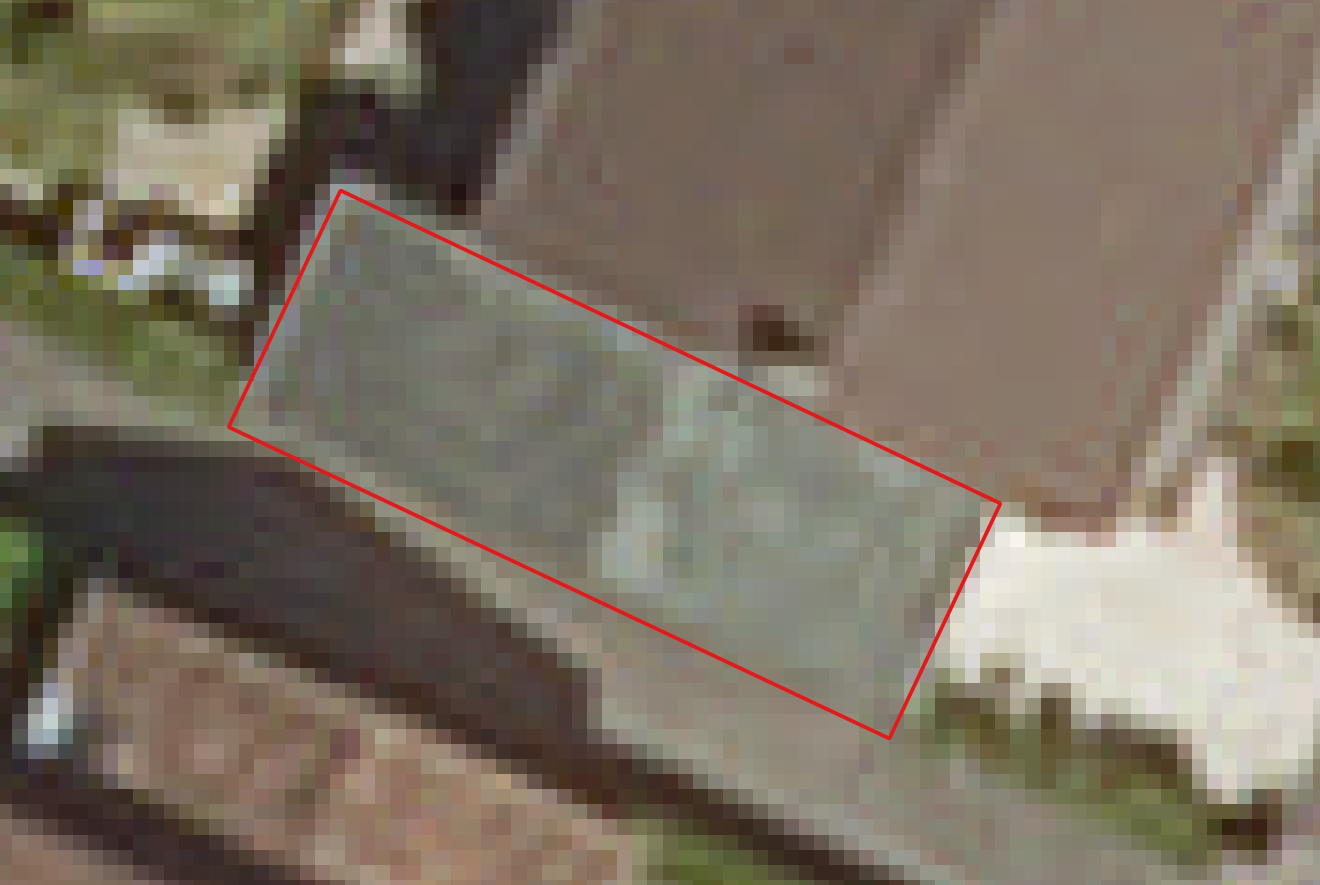
\includegraphics[height=.11\textheight]{images/Facet_Errors/under_segmentation}}
                        \ffigbox[\FBwidth]{\caption{Over segmentation}\label{fig::over_fac}}{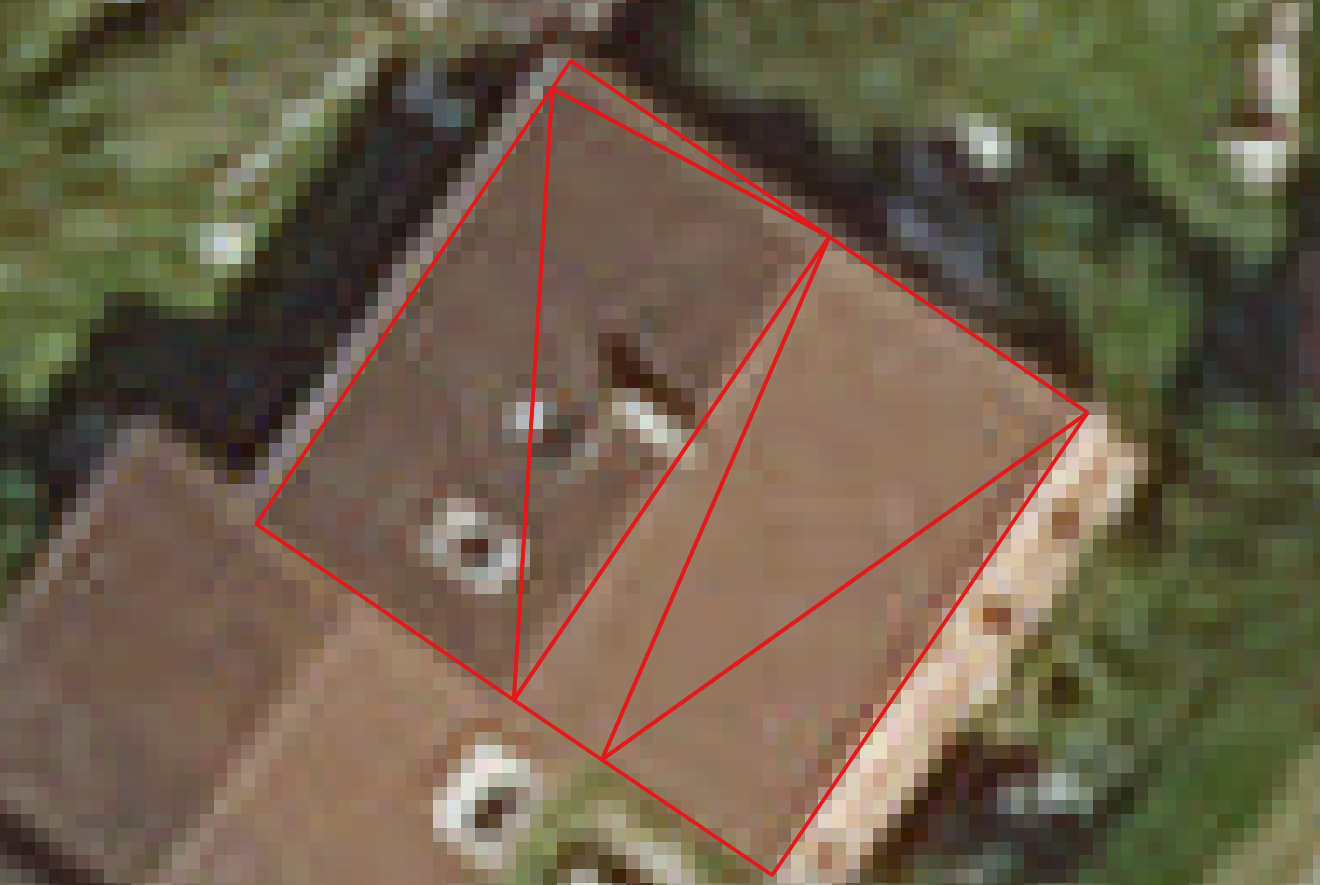
\includegraphics[height=.11\textheight]{images/Facet_Errors/over_segmentation}}
                        \ffigbox[\FBwidth]{\caption{Inexact segmentation}\label{fig::mis}}{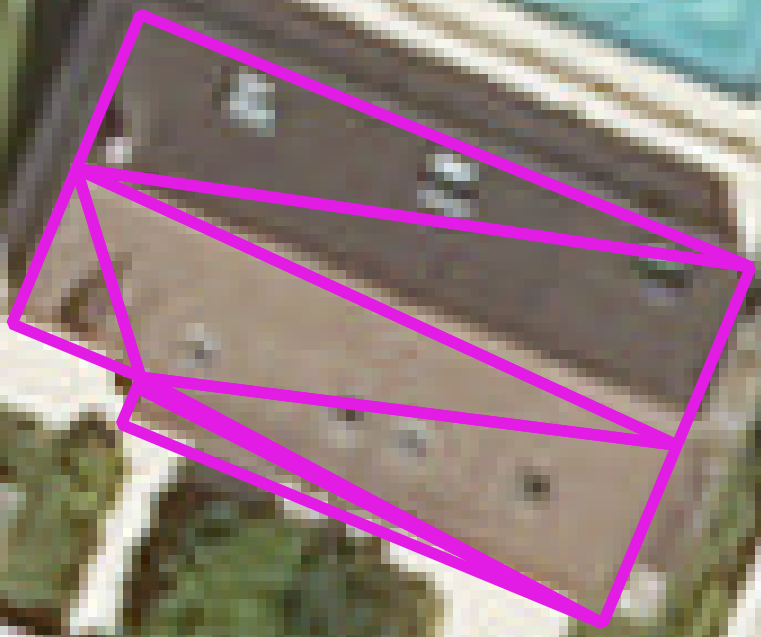
\includegraphics[height=.11\textheight]{images/Facet_Errors/mis_segmentation}}
                        \ffigbox[\FBwidth]{\caption{Imprecise slope}\label{fig::slope}}{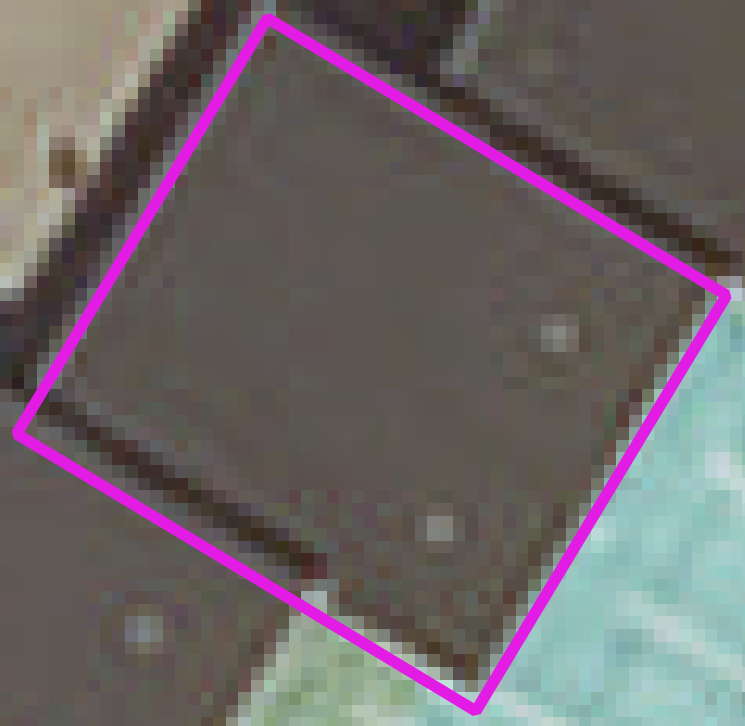
\includegraphics[height=.11\textheight]{images/Facet_Errors/slope}}
                    \end{subfloatrow}
                }
                {
                	\captionsetup{labelfont={bf},justification=raggedright, labelsep=period}
                    \renewcommand{\thesubfigure}{\roman{SubFigCounter}}

                    \captionof{subfigure}{Facet errors family samples.}\label{fig::fac_err}
                    \refstepcounter{SubFigCounter}
                    \addtocounter{figure}{-1}
                }
            }
            {
                \caption{\label{fig::samples}Error samples illustration.}
            }
        \end{center}
        \vspace{-4.5em}
    \end{figure}

\subsection{Features baseline}
In order to predict errors, models need to be described using relevant attributes. Since there is no comparable work predicting the described errors, this work proposes a baseline of features. They are kept simple, based on depth map comparison, segment and image gradient pairing or model intrinsic geometrical characteristics. The idea is to avoid computing $3D$ lines~\cite{Michelin2013}, correlation scores~\cite{boudet2006supervised} or, in general, any greedy image matching based method. In addition, these are methodologically endogamous to the $3D$ reconstruction techniques used to produce the same assessed models. In consequence, they can completely miss aspects of the reconstituted model evaluation.

The presented approach offers another degree of freedom regarding the input data to be used in model evaluation. The model itself can be of use in order to discover errors based on its geometry compared to the dataset statistics. Depth information can be added, through a \acrshort{acr::dsm}, in order to help detecting defects, especially depth related ones. Last but not least, orthorectified images can bring additional information critical for semantic heavy segmentation evaluation. Each modality is described herein in detail.

\noindent
\textbf{Geometric features.}
The model facet set is denoted by $\mathsf{F}$. $\forall (f, g) \in \mathsf{F} \times \mathsf{F} \quad f \sim g$ correspond to facets $f$ and $g$ being adjacent: \textit{i.e.} they share a common edge. As the roof topology graph in~\cite{Verma2006}, the input building model can be seen as a facet (dual) graph:
\begin{equation}
	\label{eq::model_graph}
	\mathsf{M} \equiv \Big(\mathsf{F}, \mathsf{E} \triangleq \big\{ (f, g) \in \mathsf{F} \times \mathsf{F} : f \sim g \big\} \Big)
\end{equation}
For each facet $f \in \mathsf{F}$, we compute its degree (\textit{i.e.} number of vertices; $d(f) \triangleq \vert\{v : v\text{ is a vertex of }f\}\vert$), its area $\mathscr{A}(f)$, the circumference $\mathscr{C}(f)$, the centroid $\mathscr{G}(f)$ and the normal $\vec{n}(f)$. Statistical characteristics are then computed over building model facets using specific functions $S$, like a histogram $S^p_{hist}: l \mapsto histogram(l, p)$, where $p$ represent histogram parameters, or simply $S_{synth}: l \mapsto \begin{bmatrix}
\max(l)& \min(l) & \bar{l} & \text{median}(l) & \sigma(l)
\end{bmatrix}$ where $\bar{l}$ (resp. $\sigma(l)$) represents the mean (\textit{resp.} the standard deviation) over a tuple $l$.

Each building $\mathsf{M}$ can consequently be characterized by a geometric feature vector that accounts for its geometric characteristics:

\begin{equation}
	\label{eq::geom_feat}
    v_{geometric}(\mathsf{M}) = \begin{bmatrix}
    	S \Big(\big(d(f)\big)_{f \in \mathsf{F}}\Big)\\
    	S \Big(\big(\mathscr{A}(f)\big)_{f \in \mathsf{F}}\Big)\\
    	S \Big(\big(\mathscr{C}(f)\big)_{f \in \mathsf{F}}\Big)\\
    	S \Big(\big( \vert\vert \mathscr{G}(f) - \mathscr{G}(g) \vert\vert \big)_{(f,g) \in \mathsf{E}}\Big)\\
    	S\Big(\big( \arccos(\vec{n}(f), \vec{n}(g)) \big)_{(f,g) \in \mathsf{E}}\Big)
    \end{bmatrix}
\end{equation}
Additionally to individual facet statistics, regularities are taken into account by looking into adjacent graph nodes as in~\cite{Zhou2012}. These features expresses only a small part of structural information. Taking this type of information into account would implicate graph comparisons which are not genuinely simple tasks to achieve. Since the objective is to build a baseline, this approach has not been considered for the moment.

\noindent
\textbf{Altimetric features.}
For this modality, the depth information is provided as a $2D$ height grid $dsm$. It must have been produced at the same time of the $3D$ reconstruction so as to avoid time dynamics. It is compared to the model altimetry like in~\cite{Bredif2007}. The later can be inferred from its facets plane equations. It is then rasterized into the image $alt$ at the spatial resolution of the $dsm$. Their difference reveals a discrepancy map that can be exploited for the prediction (\textit{c.f.} Figure~\ref{fig::pipeline}.c). A baseline approach is proposed relying on pixel values statistics computed using previously defined functions $S$.
\begin{equation}
	\label{eq::alti_feat}
    v_{altimetric}(\mathsf{M}) = S\big( \mathrm{vec}(dsm - alt) \big)
\end{equation}
Equation~\ref{eq::alti_feat} summarizes how building altimetric features are computed. The $\mathrm{vec}$ operator represents the matrix vectorization operator. Different from a root mean square metric~\cite{lafarge2012creating},~\cite{Poullis2013}, the histogram captures the the discrepancy distribution. However, like the previous geometric attributes, this mapping loses structural information coming from the model.

\noindent
\textbf{Image features.}
Building edges correspond to sharp discontinuities in images~\cite{canny1986computational}. The idea is to compare these edges to local gradients in order to look for inconsistencies. In an ideal setting, in an image $I$, gradients computed at pixels $g$ that intersect any segment $s$ from the building projection (\ref{fig::radio}) will almost be collinear with its normal. In consequence, we qualify, using the same statistical functions $S$, the distribution of the normalized gradient scalar product with the normal all along a segment:
\begin{equation}
	\label{eq::corr_seg}
    \mathsf{D}_S(s, I) \triangleq S \bigg( \Big(\frac{\nabla I(g) \cdot \vec{n}(s)}{\Vert \nabla I(g)\Vert})_{g \in I \textrm{ and } g \cap s} \Big)\bigg)
\end{equation}

\begin{figure}
	\begin{center}
    	\floatbox{figure}{
            \begin{subfloatrow}[2]
                \ffigbox[\FBwidth]{\caption{\tiny The building projection compared to the orthoimage.}\label{fig::radio}}{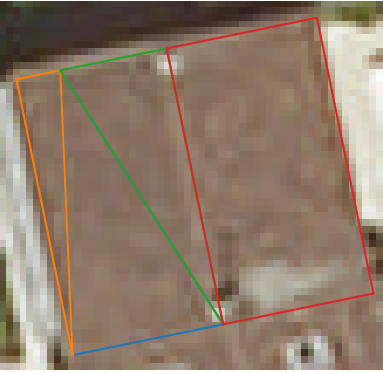
\includegraphics[width=.25\textwidth]{images/radio_vector}}
                \quad
                \ffigbox[\FBwidth]{\caption{\tiny The green squares represent intersecting pixels with the red segment. The gradient vector in purple is compared to the segment normal in black.}\label{fig::seg_inter}}{\includestandalone[mode=buildnew, width=.25\textwidth]{radiometric_features}}
            \end{subfloatrow}
        }{
        	\caption{Image features illustration.} \label{fig::image}
        }
	\end{center}
\end{figure}

Once the distribution is computed over a segment, it is compiled over all facet edges to define the distribution over projected facets. In the case of histograms $S_{hist}^p$ with the same parameters (and thus the same bins), it is equivalent to summing out the previous vectors $\mathsf{D}_{S_{hist}^p}(s, I)$ over segments $s$ forming the polygon projection $q(f)$ of the facet $f$ on as the image $I$. In order to take into account the variability of segment dimensions, this sum is weighted by segment lengths.
\begin{equation}
	\label{eq::corr_fac}
	D_{S_{hist}^p}(f, I) \triangleq \sum_{s \in q(f)} \Vert s \Vert \cdot \mathsf{D}_{S_{hist}^p}(s, I)
\end{equation}

The same reduction can be done over all facets of a building $\mathsf{M}$, resulting in equation ~\ref{eq::corr_bul}. The weights are added in order to take into account the geometry heterogeneity as well as the image. The gradient to normal comparison is similar to the $3D$ data fitting term formulation in~\cite{li2016boxfitting}. Once again, the structure of the model is lost when simply summing over all segments.
\begin{equation}
	\label{eq::corr_bul}
	v_{image}(\mathsf{M}) = D_{S_{hist}^p}(\mathsf{M}, I) \triangleq \sum_{f \in \mathsf{F}} \mathscr{A}(q(f)) \cdot \mathsf{D}_{S_{hist}^p}(f, I)
\end{equation}

\subsection{Classification process}

Two sources of flexibility are to be taken into account: the parametric nature of the taxonomy and the feature vector heterogeneity. The first means that labels to predict are not fixed but depend on the specified parameters. The second means that the classifier must adapt well to different input vectors types and sizes.

\noindent
\textbf{Classification problems.}
Both the classification problem nature and the set of labels to work with are determined by the three previously defined taxonomy parameters (\textit{c.f.} Table~\ref{tab::problems}). The first \textbf{target \textit{finesse}} $= 1$ level corresponds to a binary classification problem: Valid or Error. At the next one $\textit{finesse}=2$, the other parameters intervene. The \textbf{\acrshort{acr::elod}} can take then two values in the aerial reconstruction case: $\acrshort{acr::lod}1$ or $\acrshort{acr::lod}2$. If fixed at $\acrshort{acr::lod}1$, it is a binary classification problem: Valid or Building error. For $\acrshort{acr::lod}2$, and if the \textbf{exclusivity} is on, then it is a multi-class problem: Valid, Building error or Facet errors, while, if set off, it becomes a multi-label one: Valid, Building error and Facet errors. At the last $\textit{finesse}=3$ level, if the \textbf{exclusivity} is on, it is a $2$-stage classification problem. In the first stage, a multi-class, or simply binary in case $\acrshort{acr::elod} = \acrshort{acr::lod}1$, problem, like in the previous semantic degree, predicts the error family, after which a second multi-label problem decides between the predicted error family children. If the \textbf{exclusivity} is off, it is a $1$-stage multi-label problem that guesses the existence of each atomic error corresponding to the chosen \acrshort{acr::elod}.

\begin{table}
	\begin{center}
		\begin{tabular}{c c c x{8cm}}
			\toprule
            \textbf{\textit{finesse}} & \textbf{\acrshort{acr::elod}} & \textbf{exclusivity} & \textbf{Classification output}\\
            \midrule
            \scriptsize
            $1$ & -- & -- & Binary(Valid, Erroneous)\\
            $2$ & $\acrshort{acr::lod}1$ & -- & Binary(Valid, Building error)\\
            $2$ & $\acrshort{acr::lod}2$ & on & MultiClass(Valid, Building error, Facet error)\\
            $2$ & $\acrshort{acr::lod}2$ & off & MultiLabel(Valid, Building error, Facet error)\\
            $3$ & $\acrshort{acr::lod}1$ & on & MultiLabel(children(Binary(Valid, Building error)))\\
            $3$ & $\acrshort{acr::lod}2$ & on & MultiLabel(children(MultiClass(Valid, Building error, Facet error)))\\
            $3$ & $\acrshort{acr::lod}1$ & off & MultiLabel(children(Building error))\\
            $3$ & $\acrshort{acr::lod}2$ & off & MultiLabel(children(Building error)$\cup$ children(Facet error))\\
            \bottomrule
		\end{tabular}
        \caption{\label{tab::problems} All possible classification problem types summary. children($error$) lists $error$ children in the taxonomy tree (Figure~\ref{fig::taxonomy}).}
	\end{center}
\end{table}

In a multi-class classification problem, each instance has only one label that can take multiple values (or two in the special case of binary classification) and only one is chosen. The multi-label problem decides, for multiple labels, the most probable state: present ($+1$) or absent ($-1$). In the multi-stage setting, one decides, at each level, the most probable class or labels which impact the next stages of prediction. Errors are easily propagated in the last case. That is why, the rest of the study is not interested in this case. Since it focuses on semantic evaluation, the first \textit{finesse} degree is not experimented on. Furthermore, it can be inferred from higher levels of \textit{finesse}.

\noindent
\textbf{Classifier choice.} The highly modular nature of proposed features and the high number of parameters to study restrict the choice of classifiers. Random forest classifiers~\cite{breiman2001random} were retained in this setting. In fact, they can manage a great number of features with different types and different dynamics. It can also perform embedded feature selection that can be used to assess the added value of each type of feature. Relying on bagging strategy, a high number of trees ($1000$ elements) is necessary to cover most of the feature space and a weak tree depth ($4$) to help avoiding overfitting during training. It adapts also to any classification paradigm: multi-class or multi-label. In the later case, a one-vs-all approach is adopted in addition so as to address each label differently.
\section{Experiments}
\subsection{Data}

The used dataset results from an urban reconstruction algorithm over Elancourt (France). The studied scene spans an area of around \SI{15}{\km\squared}. It contains a stadium, a petrol station, residential districts with mostly bi-level buildings, industrial areas with flat roof buildings and administrative edifices such as schools. These were modeled, using the algorithm described in~\cite{Durupt2006}, out of footprints and an aerial photogrammetric \acrshort{acr::dsm} with a \SI{0.06}{\m} spatial resolution. This method simulates possible roof structures with constraints on facet dimensions. The best roof structure is selected after scoring the extrapolated roofs. Finally, orthogonal building fa\c{c}ades connect the best roof to the ground. The produced $2.5D$ models have a $\acrshort{acr::lod}2$ level.  $1501$ buildings are considered in these experiments. They were annotated according to the atomic errors list provided by our taxonomy. Table~\ref{tab::statistics} reports these error statistics over the annotated dataset.

\begin{table}
    \scriptsize
    \begin{center}
        \begin{tabular}{|x{1.8cm} | x{1.8cm} | x{3cm} | x{2.8cm} | x{2.5cm}|}
            \hline
            \multicolumn{1}{|c|}{\textbf{Error Family}} & \textbf{Occurrence ratio} & \textbf{\emph{Atomic} error} & \textbf{Family conditional occurrence ratio} & \textbf{Absolute occurrence ratio} \\
            \hline
            Unqualifiable & $0.0180$ & -- & -- & -- \\
            \hline
            \hline
            \multirow{4}{*}{Building Errors} & \multirow{4}{*}{$0.8235$} & Over segmentation & $0.8285$ & $0.6822$\\
            \cline{3-5}
                &                   & Under segmentation & $0.2824$ & $0.2325$ \\
            \cline{3-5}
                &                   & Imprecise footprint & $0.1521$ & $0.1252$ \\
            \cline{3-5}
                &                   & Imprecise height & $0.0057$ & $0.0047$ \\
            \hline
            \hline
            \multirow{4}{*}{Facet Errors} & \multirow{4}{*}{$0.7249$} & Over segmentation & $0.8971$ & $0.6502$ \\
            \cline{3-5}
                &                   & Under segmentation & $0.1314$ & $0.0953$ \\
            \cline{3-5}
                &                   & Imprecise segmentation & $0.1351$ & $0.9793$ \\
            \cline{3-5}
                &                   & Imprecise slope & $0.0193$ & $0.0140$ \\
            \hline
        \end{tabular}
        \caption{\label{tab::statistics} Ground truth statistics over the dataset containing $1501$ buildings.}
    \end{center}
\end{table}

Both error families are highly present in the dataset. Only a small portion ($27$ samples) of instances are unqualifiable, being occluded, completely or partially, by vegetation. At the atomic level, except building and facet over segmentation case, most errors are under represented with an extreme case of height imprecision error tally of $7$. The way dataset unbalanced nature effect on test results will be highlighted later in experiment results.
\subsection{Results}

\begin{table}
	\scriptsize
	\begin{center}
        \begin{tabular}{|x{1.4cm} | x{1.2cm} x{1.2cm} | x{1.2cm} x{1.2cm} | x{1.2cm} x{1.2cm} | x{1.2cm} x{1.2cm}|}
			\hline
            &\multicolumn{2}{x{2.4cm}|}{\textbf{Geom. feats.}} & \multicolumn{2}{x{2.4cm}|}{\textbf{Geom. \& Alti. feats.}} & \multicolumn{2}{x{2.4cm}|}{\textbf{Geom. \& Radio. feats.}} & \multicolumn{2}{|x{2.4cm}|}{\textbf{All feats.}}\\
            \cline{2-9}
            &\textbf{Recall} & \textbf{Prec.} & \textbf{Recall} & \textbf{Prec.} & \textbf{Recall} & \textbf{Prec.} & \textbf{Recall} & \textbf{Prec.}\\
            \hline
            Building errors & $0.9976$ & \textbf{0.8416} & $0.9976$ & $0.8411$& $0.9992$ & $0.8384$ & \textbf{1} & $0.8385$ \\
            \hline
            Facet errors & $0.9081$ & $0.9802$ & \textbf{0.9108} & \textbf{0.9841} & $0.9044$ & $0.9762$ & $0.9053$ & $0.9782$ \\
            \hline
		\end{tabular}
	\end{center}
    \caption{\label{tab::f2_res}Test results reported for $\textit{finesse}=2$.}
\end{table}

Based on the devised pipeline, four feature configurations were tested: ``geometric features'' only, ``geometric and altimetric features'', ``geometric and image features'' as well as ``geometric, altimetric and image features''. Each feature modality produces a $20$ dimension vector. A \SI{0.06}{\m} spatial resolution \acrshort{acr::dsm} and an orthorectified image with \SI{0.2}{\m} pixel size are used to derive altimetric and image features. Labels are extracted from a non \textbf{exclusive} and \textbf{\acrshort{acr::elod} $=\acrshort{acr::lod}2$} taxonomy. Both \textit{finesse} levels $2$ and $3$ are tested. The results are averaged over a $10$-fold cross validation tests. The overall accuracy is not interesting regarding the highly unbalanced nature of labels.
\begin{table}
	\scriptsize
	\begin{center}
        \begin{tabular}{|x{1.4cm} | x{1.2cm} x{1.2cm} | x{1.2cm} x{1.2cm} | x{1.2cm} x{1.2cm} | x{1.2cm} x{1.2cm}|}
			\hline
            &\multicolumn{2}{x{2.4cm}|}{\textbf{Geom. feats.}} & \multicolumn{2}{x{2.4cm}|}{\textbf{Geom. \& Alti. feats.}} & \multicolumn{2}{x{2.4cm}|}{\textbf{Geom. \& Radio. feats.}} & \multicolumn{2}{|x{2.4cm}|}{\textbf{All feats.}}\\
            \cline{2-9}
            &\textbf{Recall} & \textbf{Prec.} & \textbf{Recall} & \textbf{Prec.} & \textbf{Recall} & \textbf{Prec.} & \textbf{Recall} & \textbf{Prec.}\\
            \hline
            Buil. over seg & \textbf{0.9434} & $0.7709$ &$0.9336$ & \textbf{0.7766} &$0.9238$ & $0.7704$ &$0.9219$ & $0.7669$ \\
            \hline
            Buil. under seg & $0.3438$ & $0.7643$ &$0.3152$ & \textbf{0.7857} & \textbf{0.4298} & $0.7653$ &$0.4155$ & $0.7796$ \\
            \hline
            Inexact footprint & \textbf{0.2234} & \textbf{0.6885} & $0.2234$ & $0.6774$ &$0.1809$ & $0.6415$ &$0.1862$ & $0.6481$ \\
            \hline
            Imprecise height & $0$ & -- & $0$ & -- & $0$ & -- &$0.$ & $0.$ \\
            \hline
            \hline
            Fac. over seg & $0.9877$ & \textbf{0.9877} & \textbf{0.9887} & $0.9867$ &$0.9867$ & $0.9847$ &$0.9867$ & $0.9837$ \\
            \hline
            Fac. under seg & \textbf{0.0070} & \textbf{0.5} &$0.0070$ & $0.3334$ & \textbf{0.0070} & \textbf{0.5} & \textbf{0.0070} & \textbf{0.5} \\
            \hline
            Fac. inexact seg & \textbf{0.0136} & \textbf{0.6667} &$0.0136$ & $0.5$ &$0.0136$ & $0.2857$ &$0.0136$ & $0.4$ \\
            \hline
            Imprecise slope & $0$ & -- & $0$ & -- & $0$ & -- &$0$ & -- \\
            \hline
		\end{tabular}
	\end{center}
    \caption{\label{tab::f3_res}Test results reported for $\textit{finesse}=3$.}
\end{table}
\subsection{Discussion}

Results are analyzed over three criteria:
\begin{itemize}
	\item \textit{Finesse}: in terms of precision, on average $7.2\%$ is lost , at $\textit{finesse} = 3$, compared to $\textit{finesse} = 2$ (\textit{c.f.} Table~\ref{tab::f2_res}), across all features configurations, regarding ``Facet errors'' family, while only $0.6\%$ is gained, at the same level, for ``Building errors''. The same happens with regards to recall which is diminished by $2.0\%$ for ``Facet errors'' family and $8.3\%$ for the ``Building errors'' family. If determining the error family is enough then training the model at the same level is recommended.
    \item Feature configurations: results generally vary in a $2\%$ margin except in three cases. The easiest one to spot is the precision instability for facet inexact and under segmentation. This can explained by their under detection: only one or two are rightfully detected as errors while valid instances that are detected vary more between $1$ and $5$. Inexact footprint recall looses around $4\%$ in precision, when radiometric features are added, represent the second case: it could result from the poor spatial resolution of the used orthorectified image. The last and most stark one, is when radiometric features are added and Building under segmentation gains around $9\%$ in recall while loosing only around $1.5\%$. This may be explained by the high radiometric heterogeneity at building roofs.
    \item \textit{Atomic} errors: as predicted previously, errors that are well represented in the dataset achieve high recall and precision values. However, the good precision scores hide is that a big percentage of valid errors are flagged as errors as a result of their over representation. The others, being represented lower than $23\%$ of the whole, are not well detected, especially in the case of very rare errors: height imprecision ($7$) or slope errors ($21$).
\end{itemize}

\begin{figure}
	\begin{center}
    \tiny
		\begin{tabular}{| x{1.11cm} | x{.75cm} | x{.75cm} || x{1.11cm} | x{.75cm} | x{.75cm} || x{1.11cm} | x{.75cm} | x{.75cm} || x{1.11cm} | x{.75cm} | x{.75cm} |}
			\hline
			\multicolumn{3}{| c ||}{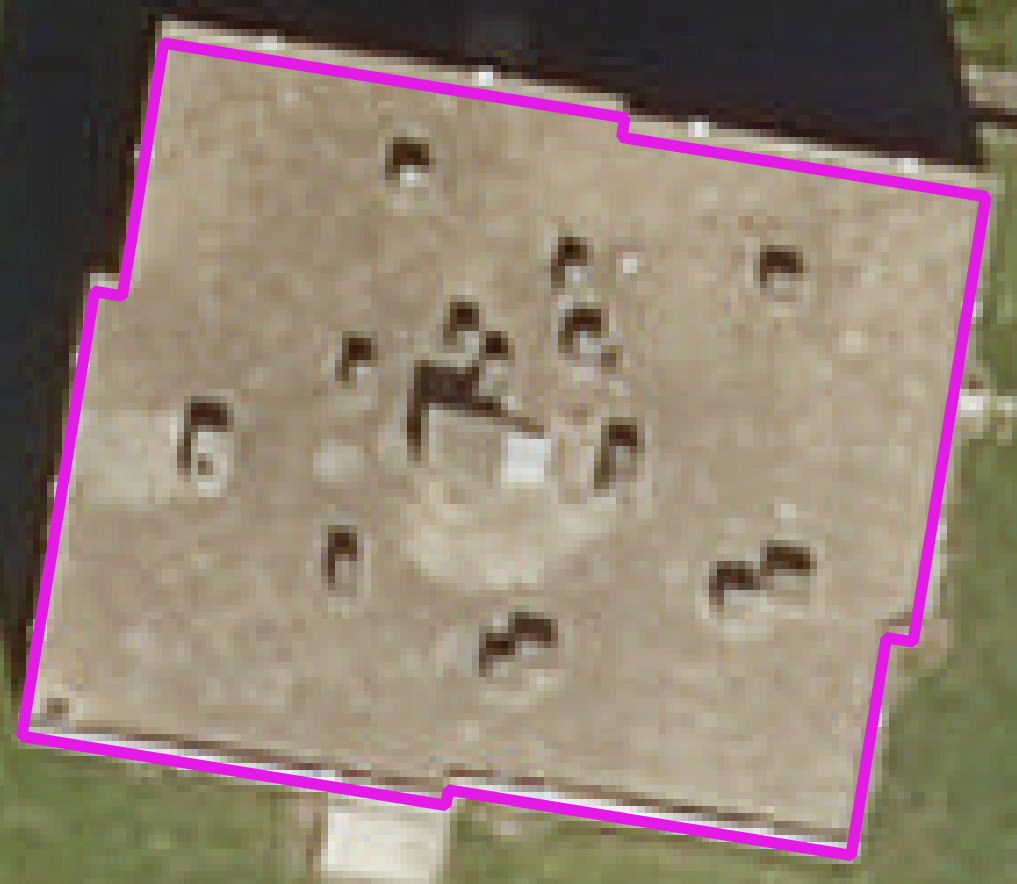
\includegraphics[height=.1\textheight,valign=m,margin=.1cm .1cm]{images/prediction_results/valid_as_bul_over}} & \multicolumn{3}{ c ||}{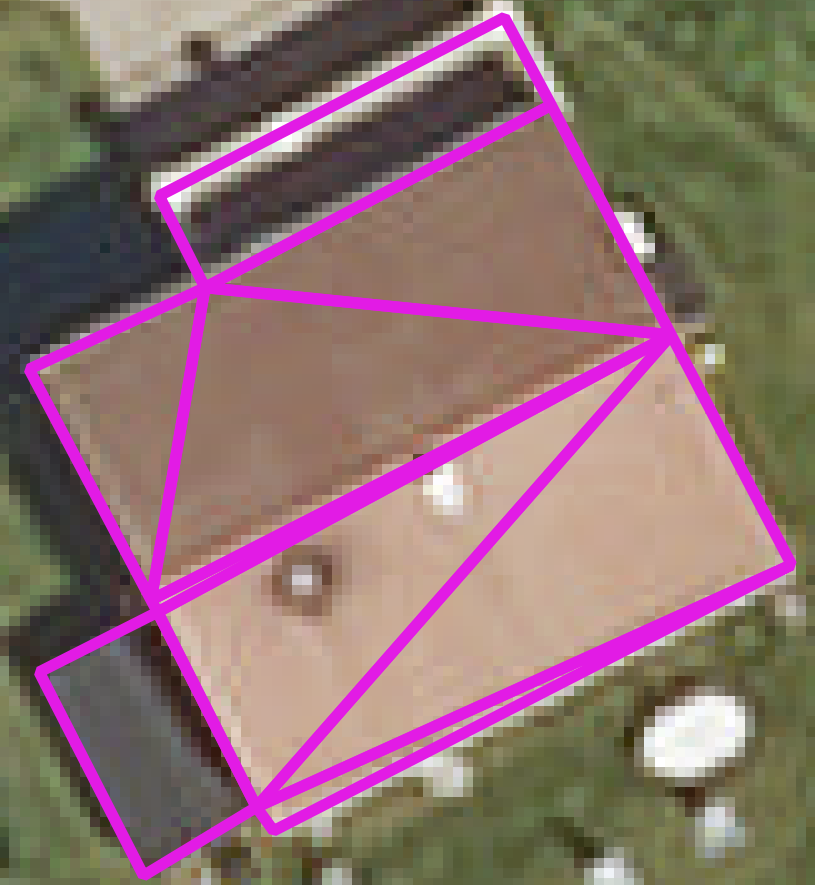
\includegraphics[height=.1\textheight,valign=m,margin=0cm .1cm]{images/prediction_results/no_imprec_no_fac_over}} & \multicolumn{3}{ c ||}{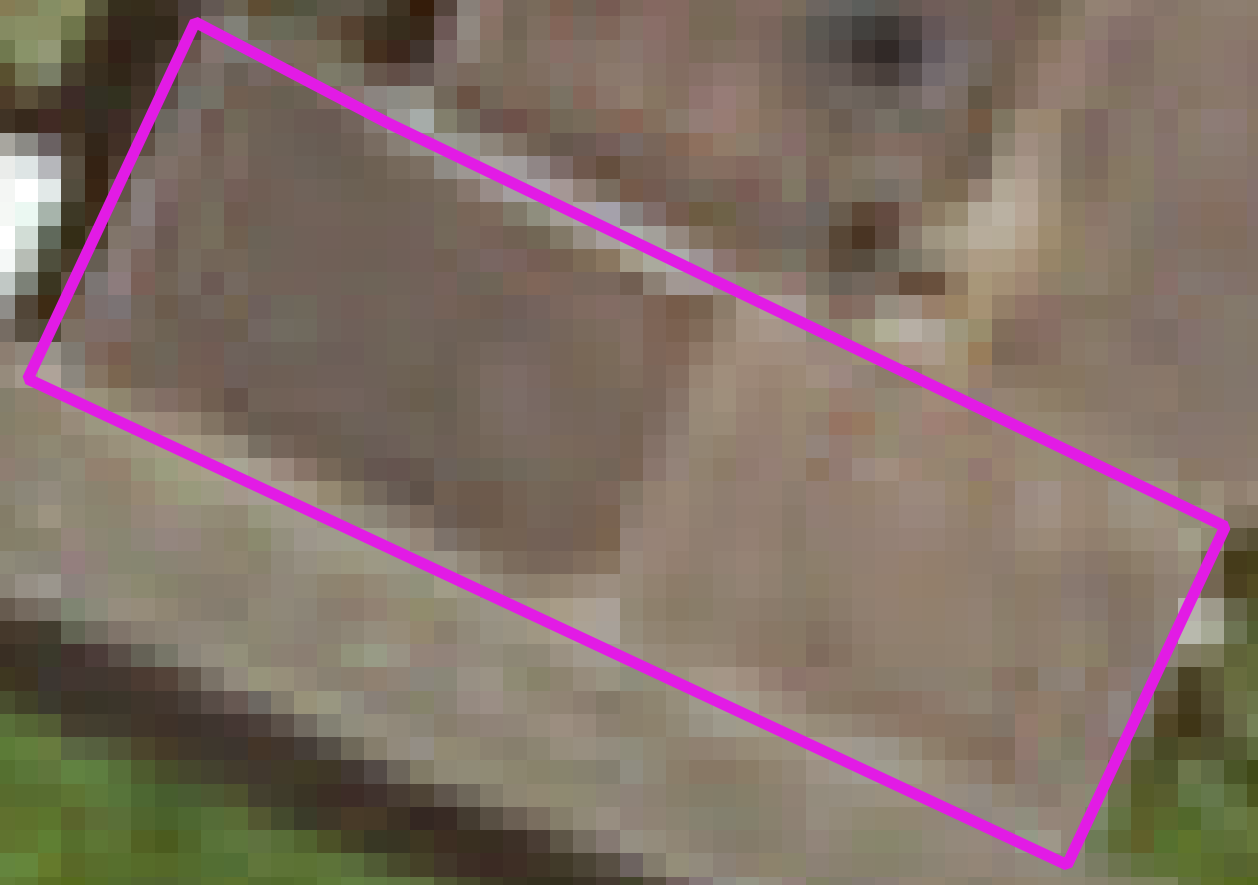
\includegraphics[height=.1\textheight,valign=m,margin=0cm .1cm]{images/prediction_results/no_under_seg}} & \multicolumn{3}{ c |}{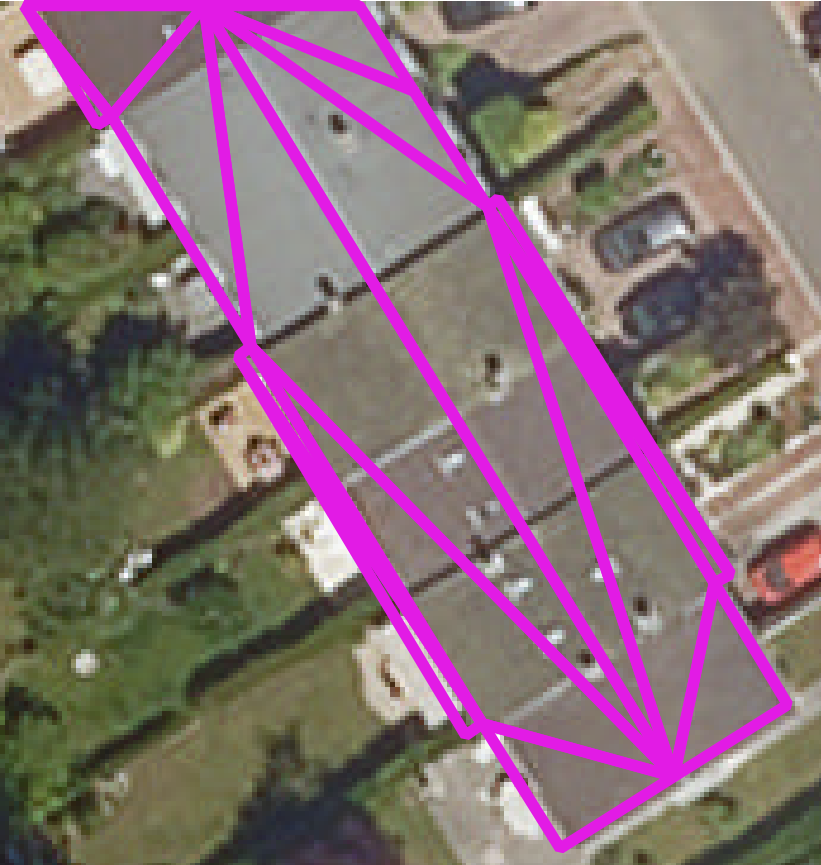
\includegraphics[height=.1\textheight,valign=m,margin=0cm .1cm]{images/prediction_results/no_bul_under_seg}} \\
			\hline
			\textbf{Errors} & \textbf{G.T.} & \textbf{Pred.} & \textbf{Errors} & \textbf{G.T.} & \textbf{Pred.} & \textbf{Errors} & \textbf{G.T.} & \textbf{Pred.} & \textbf{Errors} & \textbf{G.T.} & \textbf{Pred.}\\
            \hline
            Buil. over seg. & \xmark & \cmark & Buil. under seg. & \xmark & \cmark & Buil. over seg. & \cmark & \cmark & Buil. over seg. & \cmark & \xmark \\
            Valid & \cmark & \xmark & Fac. impr. seg. & \cmark & \xmark & Fac. under seg. & \cmark & \xmark &  Fac. over seg. & \cmark & \xmark \\
            --- & --- & --- & Fac. impr. seg. & \cmark & \xmark & --- & --- & --- & Buil. under seg. & \cmark & \xmark \\
            --- & --- & --- & --- & --- & --- & --- & --- & --- &  Footprint & \cmark & \cmark \\
            \hline
		\end{tabular}
        \caption{\label{fig::results} Predicted (Pred.) errors compared to ground truth (G.T.) labels illustrated in some pathological cases. In the first image, the building outline is similar to samples where buildings are over segmented. In the second example, the building is wrongfully detected as under segmented due to the presence of a balcony and an annex smaller building. In the third sample, while being correctly predicted as an over segmented building it fails to detect the under segmented roof. Finally, in the last depiction, except the caught footprint error, the rest are ignored as there are no such samples, in the dataset, where building over and under segmentation co-occur.}
	\end{center}
\end{figure}

\section{Conclusion}

We proposed a novel framework to semantically evaluate automatically reconstructed building models. Errors are hierarchically organized into a flexible and parametrized error taxonomy. Based on the desired \acrshort{acr::lod}, exclusivity and semantic level, an error collection is considered. Model quality is predicted then using a pretrained classifier model. Each model provides intrinsic geometrical characteristics that are compiled in a feature vector. Other modularities can help describing building models. In fact, attributes can be extracted from the comparison to images or depth data.

This new framework was applied to the case of aerial urban reconstruction. Orthorectified images and a \acrshort{acr::dsm} were used in this special for feature extraction. A dataset containing $1501$ diversified aerial reconstructed building models was experimented on using the devised evaluation method and a multimodal baseline features. Although results are mitigated over under represented errors, they are quite good on the well  persuasive enough to continue investigating the present evaluation method. The next step would be to propose more structurally aware features to apply on a richer more diverse dataset.
\bibliographystyle{splncs}
\bibliography{references}
\end{document}
